% --------------------------------------------------------------
% This is all preamble stuff that you don't have to worry about.
% Head down to where it says "Start here"
% --------------------------------------------------------------

\documentclass[12pt]{article}

\usepackage[margin=1in]{geometry}
\usepackage{amsmath,amsthm,amssymb}
\usepackage{graphicx}
\usepackage{subcaption}
\usepackage{algorithmicx}
\usepackage{algorithm}
\usepackage{algpseudocode}
\usepackage[colorlinks,linkcolor=blue]{hyperref}
\usepackage[noabbrev]{cleveref}
\usepackage{courier}
\usepackage{listings}
\usepackage{tcolorbox}

\oddsidemargin 0in
\evensidemargin 0in
\textwidth 6.5in
\topmargin -0.3in
\textheight 9.0in


\newcommand{\ignore}[1]{}
\def\pp{\par\noindent}

\newcommand{\assignment}[4]{
\thispagestyle{plain}
\newpage
\setcounter{page}{1}
\noindent
\begin{center}
\framebox{ \vbox{ \hbox to 6.28in
{CIS 4190/5190: Applied Machine Learning \hfill #1}
\vspace{4mm}
\hbox to 6.28in
{\hspace{2.5in}\large\bf\mbox{Homework #2}}
\vspace{4mm}
\hbox to 6.28in
{{\it Handed Out: #3 \hfill Due: #4}}
}}
\end{center}
}

\makeatletter
\renewcommand{\fnum@algorithm}{\fname@algorithm}
\makeatother

\lstset{basicstyle=\footnotesize\ttfamily,breaklines=true}
\lstset{framextopmargin=50pt,frame=bottomline}


\begin{document}
% --------------------------------------------------------------
%                         Start here
% --------------------------------------------------------------

\assignment{Fall 2024}{4}{11/06/2024}{11/20/2024}


\begin{itemize}
\item {\bf Your Name:}  \textit{Yueyang Li}
\item {\bf Your PennKey:} \textit{ezel22}
\item {\bf Your PennID:} \textit{47700221}
\end{itemize}

\section{Multiple Choice \& Written Questions}

\begin{enumerate}
\item
\begin{enumerate}

\item Ans
\begin{tcolorbox}
The sentence Bob will generate is: \\
"Bob loves cookie."
\end{tcolorbox}
\item Ans
\begin{tcolorbox}
    Compute the Log likelihood of "Bob loves cookies":\\
    Since \(\ln(\Pr(loves | Bob)) = -0.693 \) and \(\ln(\Pr(cookies | Bob, loves)) = -0.916 \) \\
    Therefore: \(\textbf(loglike)(\text{"Bob loves cookie"}) = -1.609\)
    
    Compute the Log likelihood of "Bob loves cookies":\\
    Since \(\ln(\Pr(hatess | Bob)) = -0.916 \) and \(\ln(\Pr(cookies | Bob, loves)) = - 1.609\) \\
    Therefore: \(\textbf(loglike)(\text{"Bob hates cookie"}) = -1.609 + (-0.916) = -2.525\)
\end{tcolorbox}
\item Ans
\begin{tcolorbox}
    \textbf{No, the greedy sampling strategy will not always give the most probable sentence.}\\
    The greedy strategy selects the most probable word at each step independently but does not consider the joint probability of the entire sequence. This can lead to suboptimal results because: \\
    Local Optima: Greedy sampling optimizes for the highest probability at each step, which may not lead to the globally most probable sentence.\\
    Sequence Dependencies: The words in the sentence are dependent on one another, and greedy sampling might miss combinations that have a higher overall probability due to lower initial probabilities.\\
    
    Here is a great example, if following the greedy choice, the algorithm will choose "Bob loves cookies" prior to "Bob loves cherry" although the later has high log-likelihood estimation.
\end{tcolorbox}
\item Ans
\begin{tcolorbox}
    we will only calculate "Bob loves Bob" and "Bob hates cookie" \\
     
    Compute the Log likelihood of "Bob loves Bob":\\
    Since \(\ln(\Pr(loves | Bob)) = -0.693 \) and \(\ln(\Pr(Bob | Bob, loves)) = - 1.386  \) \\
    Therefore: \(\textbf(loglike)(\text{"Bob loves cookie"}) = -.0693 + (-1.386) =  -2.079\)
    
    Compute the Log likelihood of "Bob hates cherry":\\
    Since \(\ln(\Pr(hatess | Bob)) = -0.916 \) and \(\ln(\Pr(cherry | Bob, hates)) = -0.357\) \\
    Therefore: \(\textbf(loglike)(\text{"Bob hates cookie"}) =-0.916 + (-0.357) = -1.273\)
    
    Therefore: \\
    The two highest log-likelihoods are:\\
    1. Bob hates cherry \\
    2. Bob loves cookie
\end{tcolorbox}
\end{enumerate}

\item
  \begin{enumerate}
  \item Ans
  \begin{tcolorbox}
    we can calculate \(E_1, E_2, E_3, E_4\) as follows:\\
    \(E_1 = (0.5 \cdot 0.7) + (0.2 \cdot 0.2) + (0.4 \cdot 0.3) + (0.1 \cdot 0.1) = 0.35 + 0.04 + 0.12 + 0.01 = 0.52\) \\
    \(E_2 = (0.5 \cdot 0.2) + (0.2 \cdot 0.7) + (0.4 \cdot 0.3) + (0.1 \cdot 0.1) = 0.1 + 0.14 + 0.12 + 0.01 = 0.37\)\\
    \(E_3 = (0.5 \cdot 0.0) + (0.2 \cdot 0.6) + (0.4 \cdot 0.4) + (0.1 \cdot 0.3) =  0 + 0.12 + 0.16 + 0.03 = 0.31\)\\
    \(E_4 = (0.5 \cdot 0.1) + (0.2 \cdot 0.1) + (0.4 \cdot 0.0) + (0.1 \cdot 0.9)= 0.05 + 0.02 + 0 + 0.09 = 0.16\)\\
    Therefore, we have \(E^{t} = [0.52, 0.37, 0.31, 0.16]\)
  \end{tcolorbox}
  

  \item Ans
  \begin{tcolorbox}
    calculate the nominators:\\
    \(e^{0.52} = 1.682\) \\
    \(e^{0.37} = 1.447\) \\
    \(e^{0.31} = 1.363\) \\
    \(e^{0.16} = 1.174\) \\
    \(e^{0.52} + e^{0.37} + e^{0.16} + e^{0.16} = 1.682 + 1.447 + 1.363 + 1.174 = 5.666\)\\
    
    Therefore: \\
    \[
        \alpha^{t} = \text{softmax}(E^{t}) =  [\frac{1.682}{5.666}, \frac{1.447}{5.666}, \frac{1.363}{5.666}, \frac{1.174}{5.666}] = [0.297, 0.255, 0.241, 0.207]
    \]
    
  \end{tcolorbox}
  \newpage
  \item Ans
  \begin{tcolorbox}
    We just have to compute the weighted sum:
    \[
    \begin{gathered}
        0.297 \cdot [0.7, 0.2, 0.3, 0.1] + 0.255 \cdot [0.2, 0.7, 0.3, 0.1] \\
        + 0.241 \cdot [0.0, 0.6, 0.4, 0.3] + 0.207 \cdot [0.1, 0.1, 0.0, 0.9]\\
        = [0.280, 0.404, 0.262, 0.314]
    \end{gathered}
    \]
  \end{tcolorbox}
  \end{enumerate}  
\item
\begin{enumerate}
    \item Ans\\
    \begin{tcolorbox}
        For this Problem \(l\) represents moving left, and \(r\) represents moving right
        \(G_t = R(f,l,e) + 1.0 * R(e, l, d) + ... + 1.0 * R(b, l, a) = 100\)\\
        \(G_t = R(f,r,g) + 1.0 * 1.0 * R(g, r, h) = 30\) \\
        Therefore, the optimal action is moving left to e.
    \end{tcolorbox}
    \item Ans\\
    \begin{tcolorbox}
        Similarily, \(\gamma = 0.5\):\\
        \(G_t = R(f,l,e) + 0.5 * R(e, l, d) + ... + 0.5^{5}* R(b, l, a) = 3.125\)\\
        \(G_t = R(f,r,g) + 1.0 * 0.5 * 0.5 * R(g, r, h) = 7.5\) \\
        Therefore, moving to the right to h is the optimal action
    \end{tcolorbox}
    
    \item Ans
    \begin{tcolorbox}
        Let's solve \(\gamma\) 
        we have to solve:
        \begin{align*}
            \gamma^{5} \cdot 100 &=  \gamma^{2} \cdot 30 \\
            \gamma^{2} \cdot (100\gamma^{3} - 30) &= 0 
        \end{align*}
        Therefore, taken \(\gamma \in \mathbb{R}\),
        \[
        \gamma = \sqrt[3]{0.3} = 0.67
        \]
    \end{tcolorbox}
    \item Ans
    \begin{tcolorbox}
        Initialization:\\
        Initialize $V(s)=0$ for all states, except $V(\text{terminal}) = 0$.\\
        Compute $V(s)$ for one complete pass through all states.\\
        \begin{align*}    
            V(b) &= \max\{100 + 1 \times 0, 0 + 1 \times 0\} &= 100\\
            V(c) &= \max\{0 + 1 \times 100, 0 + 1 \times 0\} &= 100\\
            V(d) &= \max\{0 + 1 \times 100, 0 + 1 \times 0\} &= 100\\
            V(e) &= \max\{0 + 1 \times 100, 0 + 1 \times 0\} &= 100\\
            V(f) &= \max\{0 + 1 \times 100, 0 + 1 \times 0\} &= 100\\
            V(g) &= \max\{0 + 1 \times 100, 30 + 1 \times 0\} &= 100\\     
        \end{align*}
        And besides that \(V(h) = 0\), and \(V(a) = 0\), they are not changed in the loop
    \end{tcolorbox}
    \item Ans
    \begin{tcolorbox}
        Initialize $V(s)=0$ for all states. \(V(\text{terminal}) = 0\).\\
        Compute $V(s)$ for one complete pass through all states.\\
        \begin{align*}    
            V(g) &= \max\{0 + 1 \times 0, 30 + 1 \times 0\} &= 30\\
            V(f) &= \max\{0 + 1 \times 0, 0 + 1 \times 30\} &= 30\\
            V(e) &= \max\{0 + 1 \times 0, 0 + 1 \times 30\} &= 30\\
            V(d) &= \max\{0 + 1 \times 0, 0 + 1 \times 30\} &= 30\\
            V(c) &= \max\{0 + 1 \times 0, 0 + 1 \times 30\} &= 30\\
            V(b) &= \max\{100 + 1 \times 0, 0 + 1 \times 30\} &= 100\\     
        \end{align*}
        And besides that \(V(h) = 0\), and \(V(a) = 0\), they are not changed in the loop
    \end{tcolorbox}
    
    \item Ans
    \begin{tcolorbox}
        1. \textbf{Left to Right}: In this case, \(1\) iteration since after one VI, the array will no longer update its Value functions\\
        2. \textbf{Right to Left}: In this case, \(1\) iteration since after one VI, the array will no longer update its Value functions
    \end{tcolorbox}
\end{enumerate}
\item
\begin{enumerate}
    \item Ans
    \begin{tcolorbox}
        \begin{center}
        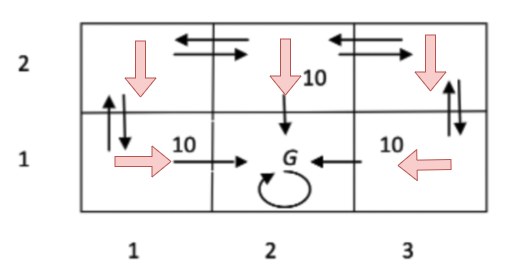
\includegraphics[scale = 0.5]{images/p4a.png}
        \end{center}
    \end{tcolorbox}
    \item Ans
    \begin{tcolorbox}
        We want to calculate \(V^{*}(1,2)\), There are two options regarding this cell.\\
        \textbf{Move Right} to cell \((2,2)\)\\
        \textbf{Move Down} to cell \((1,1)\)\\
        Therefore:
        \[
        V^{*}(1, 2) = \max \{0 + 0.8 \cdot V^{*}(2,2), 0 + 0.8 \cdot V^{*}(1,1)\}
        \]
        \textbf{First, we calculate:}  \(V^{*}(2,2)\)
        \[
        V^{*}(2, 2) = \max \{0 + 0.8 \cdot V^{*}(3,2), 10 + 0.8 \times V^{*}(G)\}
        \]
        
        We reached the absorbing state, where its value function can be caculated by:
        \[
        V^{*}(G) = \frac{R(G, a, G)}{1 - \gamma}  = 0
        \]
        Now \(V^{*}(2,2) = \max\{ 0 + 0.8 \cdot V^{*}(3,2), 10\} = 10\)
        \textbf{second, we calculate} \(V^{*}(1,1)\)
        \[
        V^{*}(1,1) = \max\{10 + 0.8 \cdot V^{*}(2,1), 0 + 0.8 \cdot V^{*}(1,2)\} = 10
        \]
        Therefore, finally, we have
        \[
        V^*(1,2) = \max\{8, 8\} = 8
        \]
        
    \end{tcolorbox}
    \item Ans
    \begin{tcolorbox}
        Premise: Q values are intialized to \(0\) , and \(\alpha\) = 0.1\\
        From the bottom-left $(1,1)$ to $G$, we would have the following loop:
$$
Q[(1,1),up] = Q[(1,1), up] + 0.1 (0 + 0.8 \max_{a^{\prime}}Q[(1,2),a^{\prime}] - Q[(1,1),up])
$$
Since $Q[(1,2),a^{\prime}] = 0$, we get:
$$
Q[(1,1), \text{up}] = 0
$$

For $Q[(1,2),\text{right}]$ , we have
$$
Q[(1,2), \text{right}] =Q[(1,2), \text{right}] + 0.1 \cdot (0 + 0.8 \max_{a^{\prime}}Q[(2,2),a^{\prime}] - Q[(1,2), \text{right}])
$$
Since $Q[(2,2), a^{\prime}] = 0$, we get:
$$
Q[(1,2), \text{right}] = 0
$$

For $Q[(3,2),\text{down}]$ , we have
$$
Q[(3,2), \text{down}] =Q[(3,2), \text{down}] + 0.1 \cdot (0 + 0.8 \max_{a^{\prime}}Q[(3,1),a^{\prime}] - Q[(3,2), \text{}])
$$
Since $Q[(2,2), a^{\prime}] = 0$, we get:
$$
Q[(3,2), \text{down}] = 0
$$

For ${} Q[(3,1),\text{left}] {}$ , we have
$$
Q[(3,1), \text{left}] =Q[(3,1), \text{left}] + 0.1 \cdot (10 + 0.8 \max_{a^{\prime}}Q[G,a^{\prime}] - Q[(3,1), \text{left}])
$$
Since we know that $Q[G, a^{\prime}] = 0$ , therefore
$$
Q[(3,1),left] = 1
$$

This terminates the current episode.
So in a nutshell, after the first episode
$$
\begin{cases}
Q[(1,1),A] &= 0 \\
Q[(1,2),A] &= 0 \\
Q[(2,2),A] &= 0 \\
Q[(3,2),A] &= 0 \\
Q[(3,1),\text{up}]&= 0 \\
Q[(3,1),\text{left}]&=1 \\
Q[(G), A] &= 0
\end{cases}
$$

\end{tcolorbox}

\end{enumerate}
\item Ans
\begin{tcolorbox}
    Further training won't solve the problem because of the reason as listed:
    \begin{itemize}
        \item The Robot receives \(+1\) rewards regardless of the step taken, there's no penalty for inefficiency, so there's no additional incentive / reward for robot to optimize the path.
        \item The robot will get stuck in a locally optimal policy that solves the maze but does not explore shorter routes. Training will reinforce the current policy.
    \end{itemize}
    Suggest fix to this problem are:
    \begin{itemize}
        \item Have Negative feedback(penalty) for every step it takes, encouraging the agent to find the shortest path.
        \item include discount factor \(\gamma < 1\) os that future rewards are worth less than immediate rewards, this will result in higher total rewards because \(\gamma^T\) decreaeses over the steps taken
    \end{itemize}
\end{tcolorbox}
\item Programming Assignment
\begin{enumerate}
    \item 2.7
    \begin{center}
    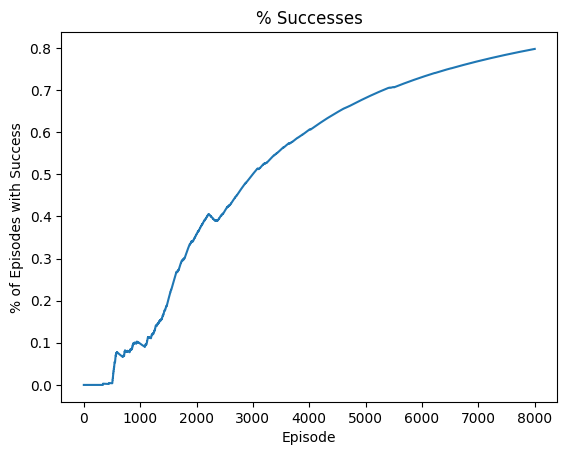
\includegraphics[scale = 0.5]{images/2.7.1.png}
    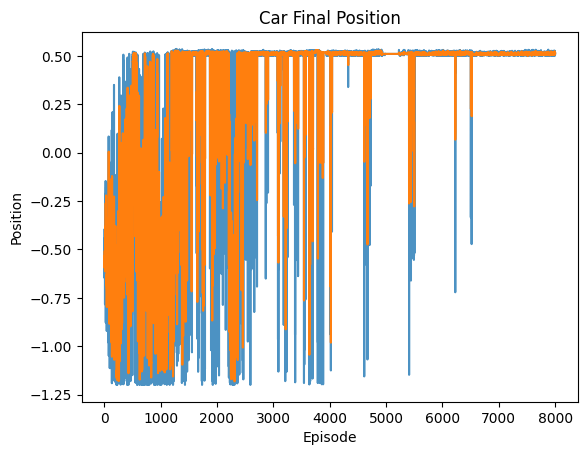
\includegraphics[scale = 0.5]{images/2.7.2.png}
    \end{center}
    \item 2.9
    \begin{center}
    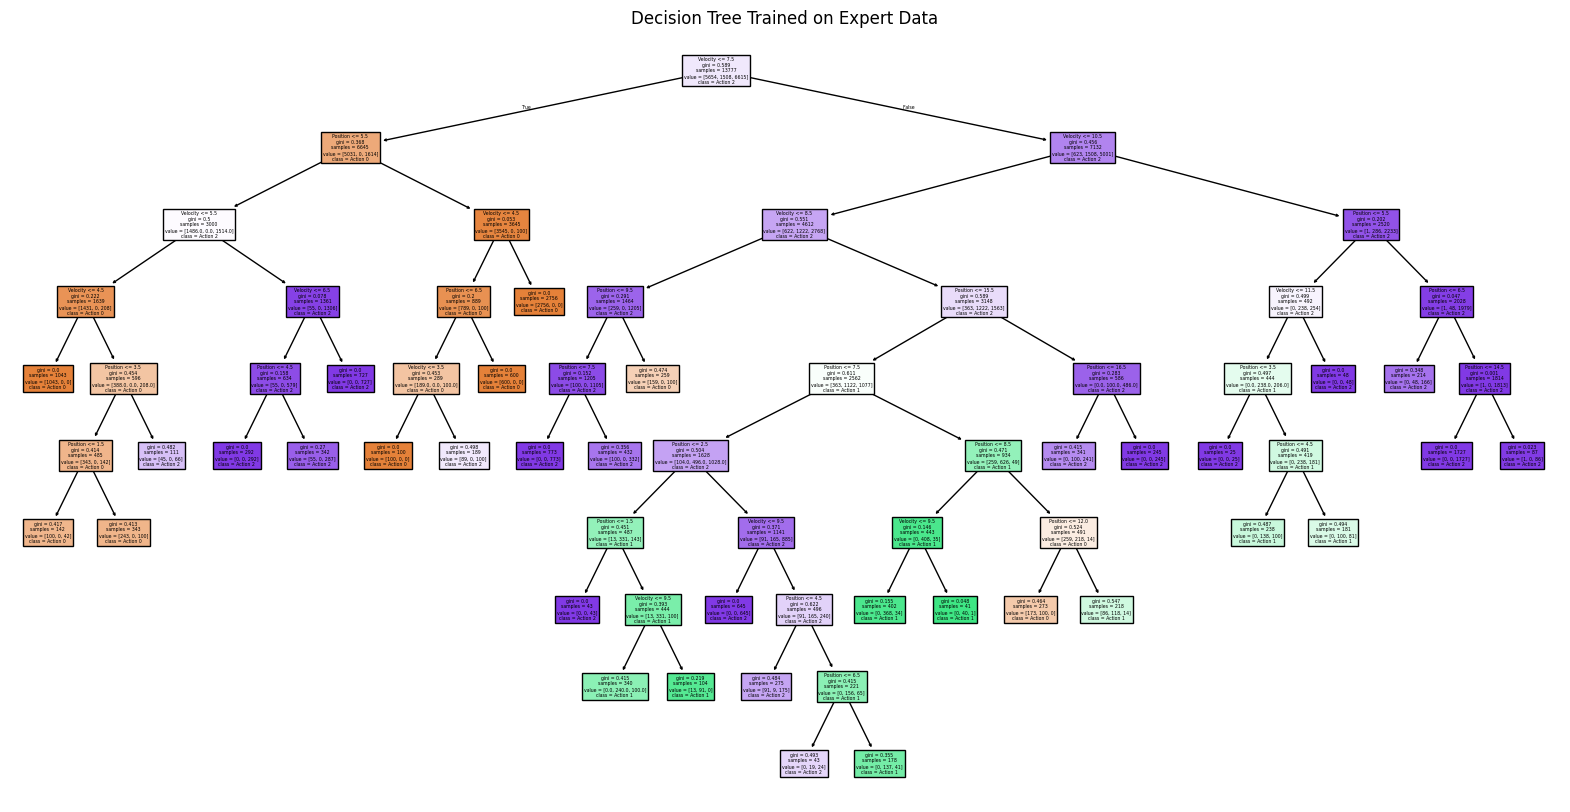
\includegraphics[scale = 0.4]{images/2.9.png}
    \end{center}
    \item 2.10
     
    \begin{center}
    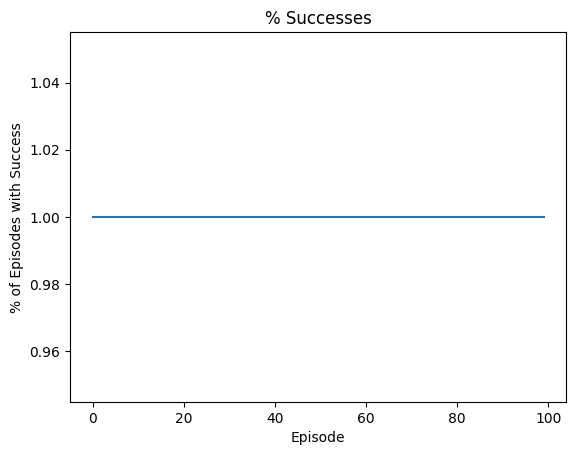
\includegraphics[scale = 0.5]{images/2.10.1.png}
    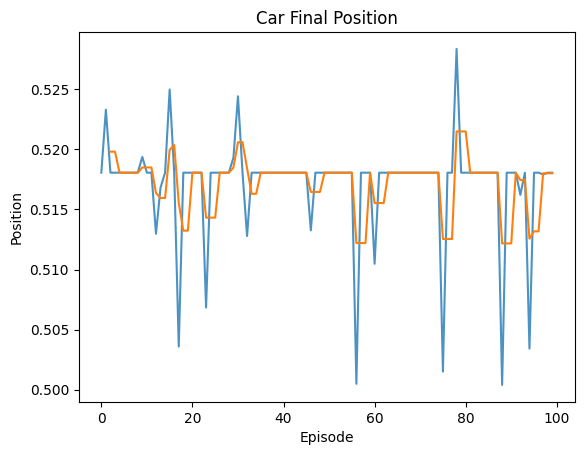
\includegraphics[scale = 0.5]{images/2.10.2.png}
    \end{center}
    \paragraph{}
    Analyze:
    Q-learning Agent: The Q-learning agent refines its policy through exploration and reward feedback, achieving increasingly stable success rates over episodes. It consistently reaches the goal (position 0.5) with minimal deviation in later episodes, demonstrating effective optimization and adaptability.\\

    Decision Tree Agent (Behavioral Cloning): The Decision Tree agent, trained on Q-learning’s data, achieves high success rates early but lacks adaptability. Its final positions vary significantly, reflecting its inability to handle novel states or refine its policy, often resulting in inefficient and unstable paths to the goal.
\end{enumerate}
\end{enumerate}
\end{document}